\documentclass[13pt,onlymath]{beamer}
\usefonttheme{serif}
\usepackage{graphicx,amsmath,amssymb,tikz,psfrag,epstopdf,fancyvrb}
\usepackage[lighttt]{lmodern}
%\usepackage{graphicx,psfrag}

\input defs.tex

%% formatting

\mode<presentation>
{
\usetheme{default}
}
\setbeamertemplate{navigation symbols}{}
\usecolortheme[rgb={0.13,0.28,0.59}]{structure}
\setbeamertemplate{itemize subitem}{--}
\setbeamertemplate{frametitle} {
    \begin{center}
      {\large\bf \insertframetitle}
    \end{center}
}

\newcommand\footlineon{
  \setbeamertemplate{footline} {
    \begin{beamercolorbox}[ht=2.5ex,dp=1.125ex,leftskip=.8cm,rightskip=.6cm]{structure}
      \footnotesize \insertsection
      \hfill
      {\insertframenumber}
    \end{beamercolorbox}
    \vskip 0.45cm
  }
}
\footlineon

\AtBeginSection[] 
{ 
    \begin{frame}<beamer> 
        \frametitle{Outline} 
        \tableofcontents[currentsection,currentsubsection] 
    \end{frame} 
} 

%% begin presentation

\title{\large \bfseries Shortest Path Algorithms}

\author{Jaehyun Park\\[3ex]
CS 97SI\\
Stanford University}

\date{\today}

\begin{document}

\frame{
\thispagestyle{empty}
\titlepage
}

\section{Cross Product}
\begin{frame}{Cross Product}
\BIT
\item Arguably the most important operation in 2D geometry
\item We'll use it all the time
\vfill
\item Applications:
\BIT
\item Determining the (signed) area of a triangle
\item Testing if three points are collinear
\item Determining the orientation of three points
\item Testing if two line segments intersect
\EIT \EIT
\end{frame}

\begin{frame}{Cross Product}
Define $\mathrm{ccw}(A, B, C) = (B-A) \times (C-A) = (b_x-a_x)(c_y-a_y)-(b_y-a_y)(c_x-a_x)$
\begin{center}
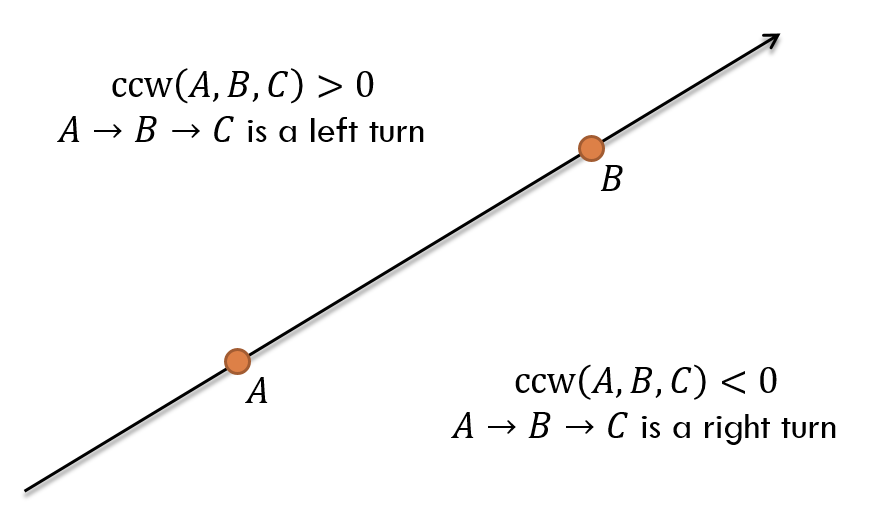
\includegraphics[height=0.5\textheight]{figures/ccw}
\end{center}
\end{frame}

\begin{frame}{Segment-Segment Intersection Test}
\BIT
\item Given two segments $AB$ and $CD$
\item Want to determine if they intersect properly: two segments meet at a single point that are strictly inside both segments
\EIT
\begin{center}
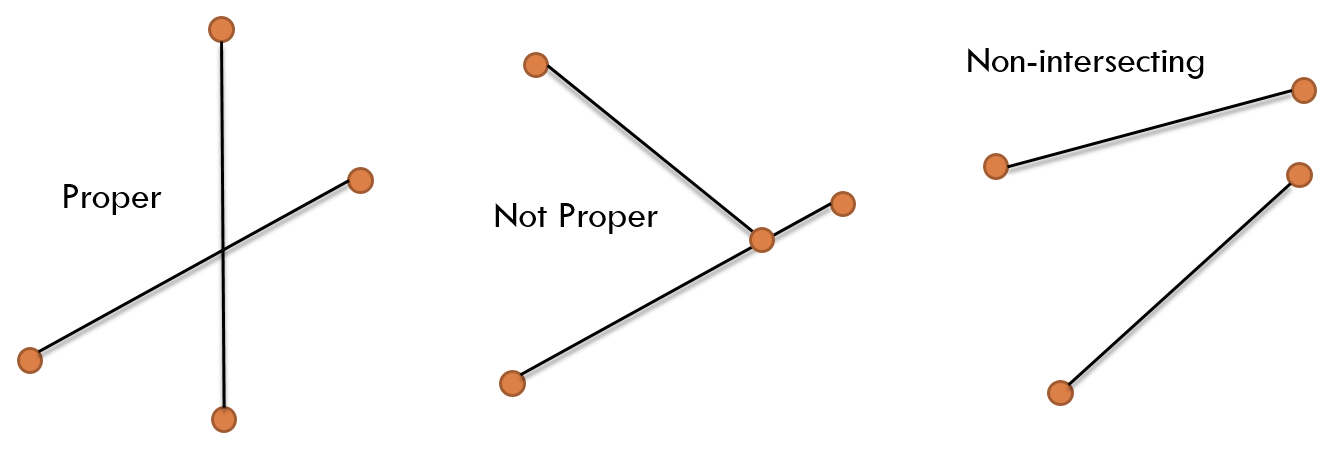
\includegraphics[width=0.8\textwidth]{figures/seg_intersection}
\end{center}
\end{frame}

\begin{frame}{Segment-Segment Intersection Test}
\BIT
\item Assume that the segments intersect
\BIT
\item From $A$'s point of view, looking straight to $B$, $C$ and $D$ must lie on different sides
\item Holds true for the other segment as well
\EIT
\item The intersection exists and is proper if:
\BIT
\item $\mathrm{ccw}(A, B, C) \times \mathrm{ccw}(A, B, D) < 0$
\item \emph{and} $\mathrm{ccw}(C, D, A) \times \mathrm{ccw}(C, D, B) < 0$
\EIT\EIT
\end{frame}

\begin{frame}{Non-proper Intersections}
\BIT
\item We need more special cases to consider!
\item \eg, If $\mathrm{ccw}(A, B, C)$, $\mathrm{ccw}(A, B, D)$, $\mathrm{ccw}(C, D, A)$, $\mathrm{ccw}(C, D, B)$ are all zeros, then two segments are collinear
\item Very careful implementation is required
\EIT
\end{frame}

\section{Convex Hull Problem}

\begin{frame}{Convex Hull Problem}
\BIT
\item Given $n$ points on the plane, find the smallest convex polygon that contains all the given points
\BIT
\item For simplicity, assume that no three points are collinear
\EIT\EIT
\begin{center}
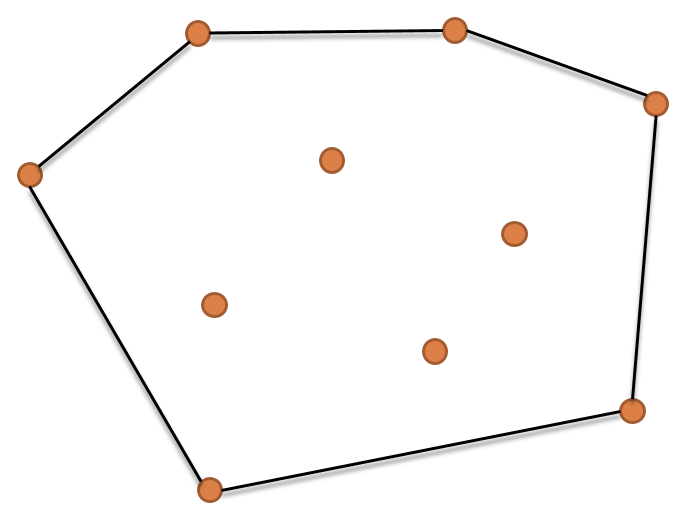
\includegraphics[height=0.5\textheight]{figures/convhull}
\end{center}
\end{frame}

\begin{frame}{Simple Algorithm}
\BIT
\item $AB$ is an edge of the convex hull iff $\mathrm{ccw}(A, B, C)$ have the same sign for all other points $C$
\BIT
\item This gives us a simple algorithm
\EIT
\vfill
\item For each $A$ and $B$:
\BIT
\item If $\mathrm{ccw}(A, B, C) > 0$ for all $C \ne A, B$:
\BIT
\item Record the edge $A \rightarrow B$
\EIT\EIT
\item Walk along the recorded edges to recover the convex hull
\EIT
\end{frame}

\begin{frame}{Faster Algorithm: Graham Scan}
\BIT
\item We know that the leftmost given point has to be in the convex hull
\BIT
\item We assume that there is a unique leftmost point
\EIT
\item Make the leftmost point the origin
\BIT
\item So that all other points have positive $x$ coordinates
\EIT
\item Sort the points in increasing order of $y/x$
\BIT
\item Increasing order of angle, whatever you like to call it
\EIT
\item Incrementally construct the convex hull using a stack
\EIT
\end{frame}

\begin{frame}{Incremental Construction}
\BIT
\item We maintain a \emph{convex chain} of the given points
\item For each $i$, do the following:
\BIT
\item Append point $i$ to the current chain
\item If the new point causes a concave corner, remove the bad vertex from the chain that causes it
\item Repeat until the new chain becomes convex
\EIT\EIT
\end{frame}

\begin{frame}{Example}
Points are numbered in increasing order of $y/x$
\begin{center}
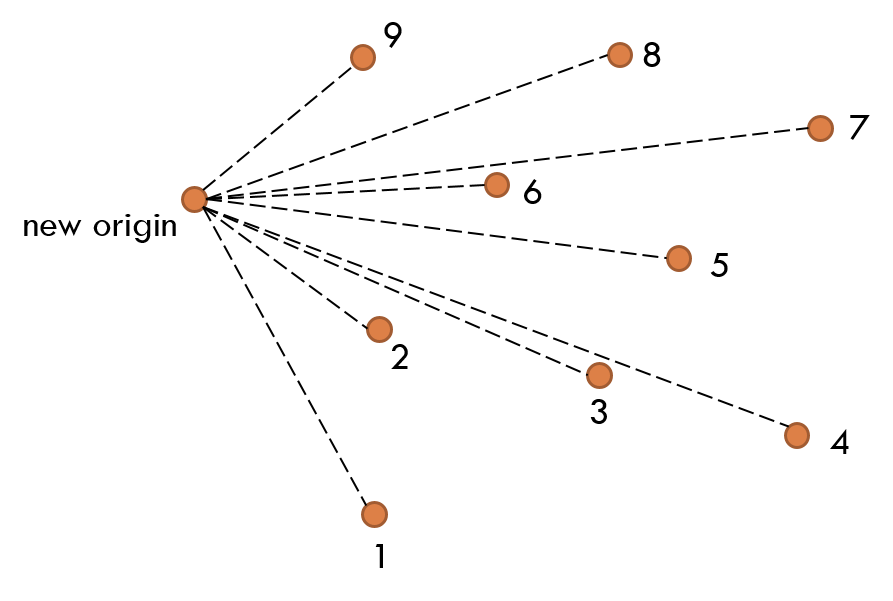
\includegraphics[height=0.5\textheight]{figures/graham1}
\end{center}
\end{frame}

\begin{frame}{Example}
Add the first two points in the chain
\begin{center}
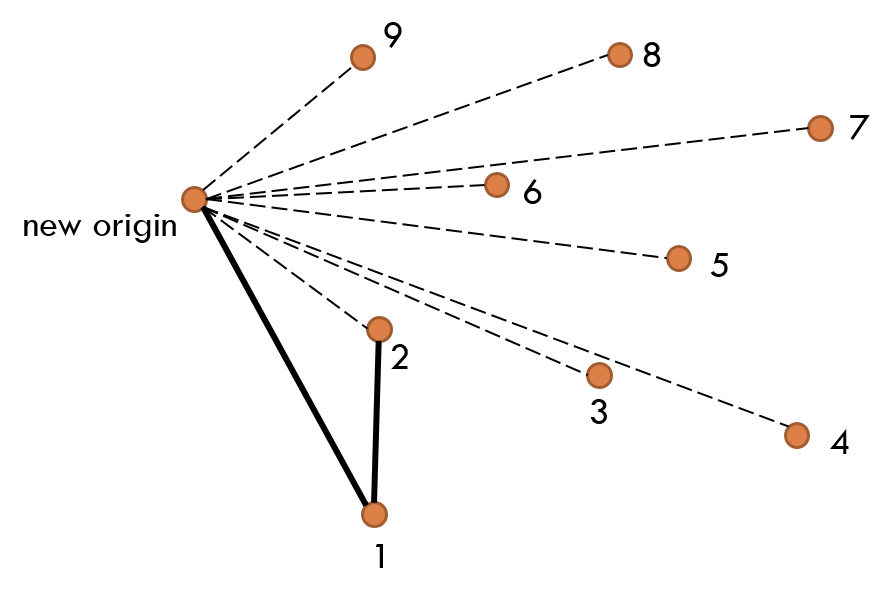
\includegraphics[height=0.5\textheight]{figures/graham2}
\end{center}
\end{frame}

\begin{frame}{Example}
Adding point 3 causes a concave corner 1-2-3: remove 2
\begin{center}
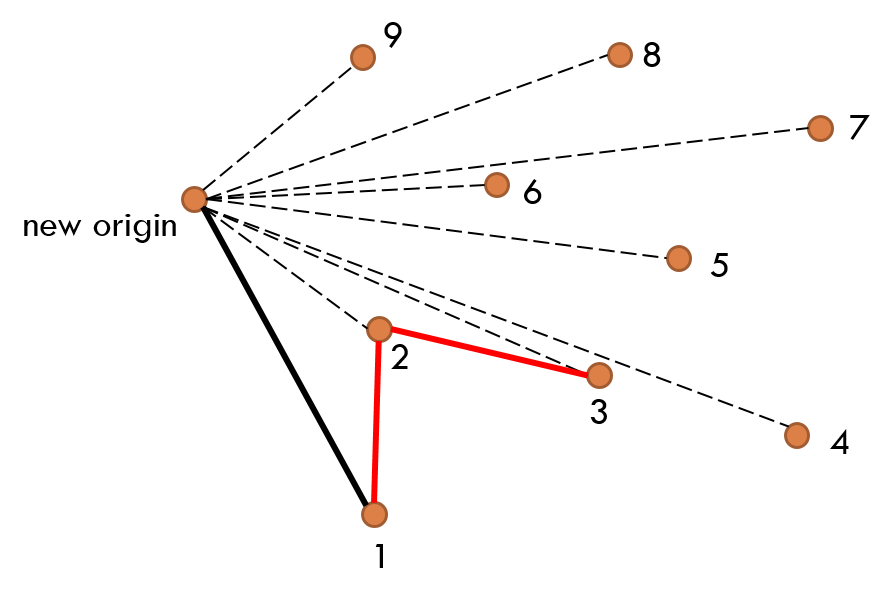
\includegraphics[height=0.5\textheight]{figures/graham3}
\end{center}
\end{frame}

\begin{frame}{Example}
That's better...
\begin{center}
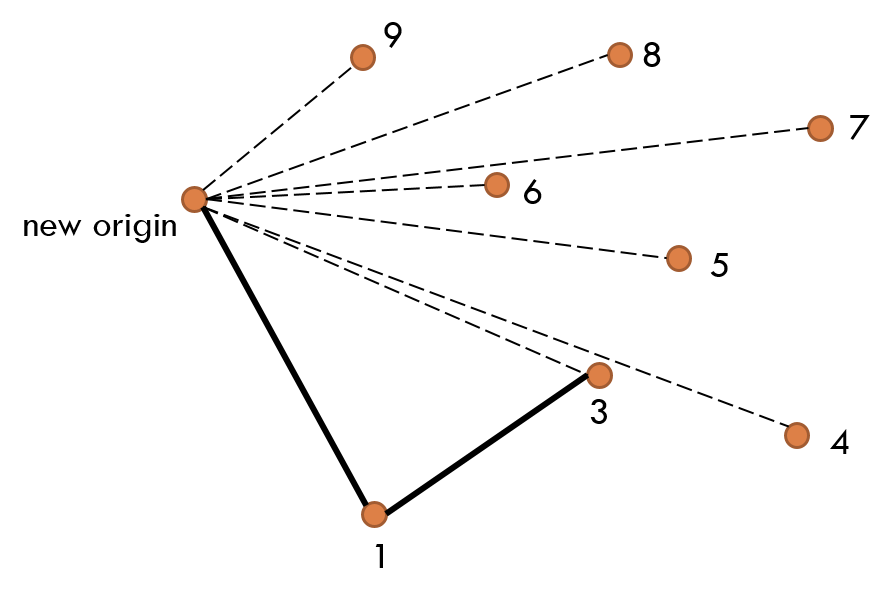
\includegraphics[height=0.5\textheight]{figures/graham4}
\end{center}
\end{frame}

\begin{frame}{Example}
Adding point 4 to the chain causes a problem: remove 3
\begin{center}
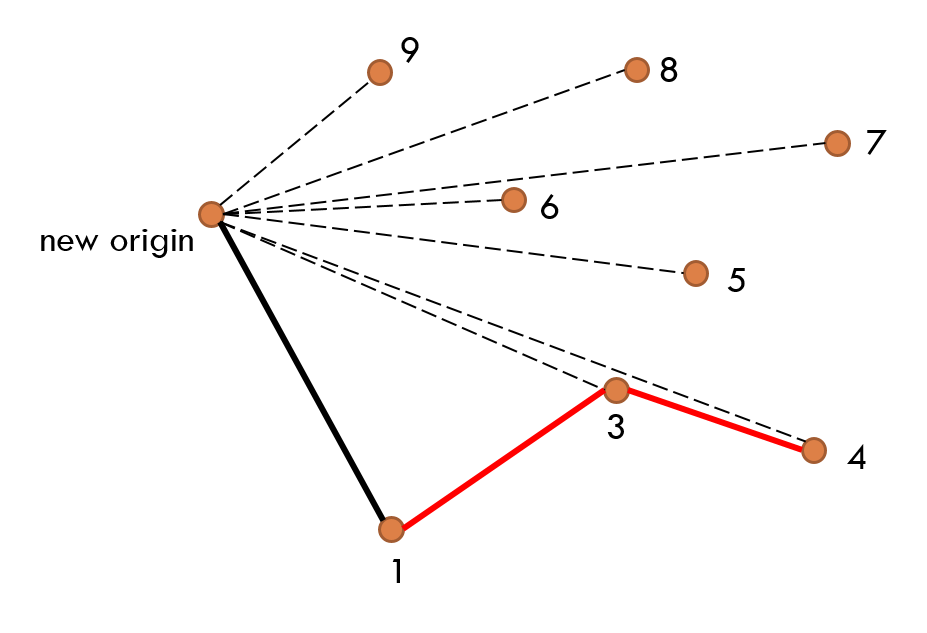
\includegraphics[height=0.5\textheight]{figures/graham5}
\end{center}
\end{frame}

\begin{frame}{Example}
Continue adding points...
\begin{center}
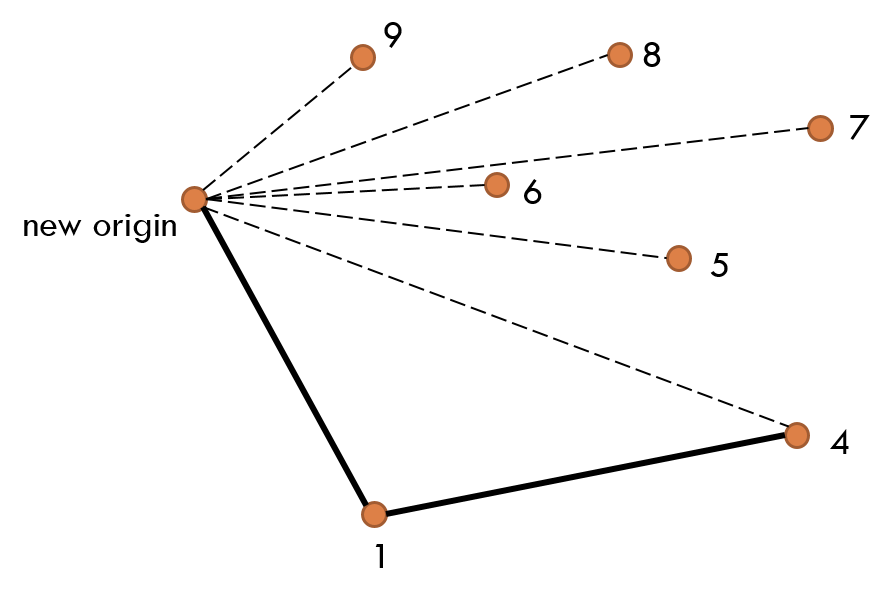
\includegraphics[height=0.5\textheight]{figures/graham6}
\end{center}
\end{frame}

\begin{frame}{Example}
Continue adding points...
\begin{center}
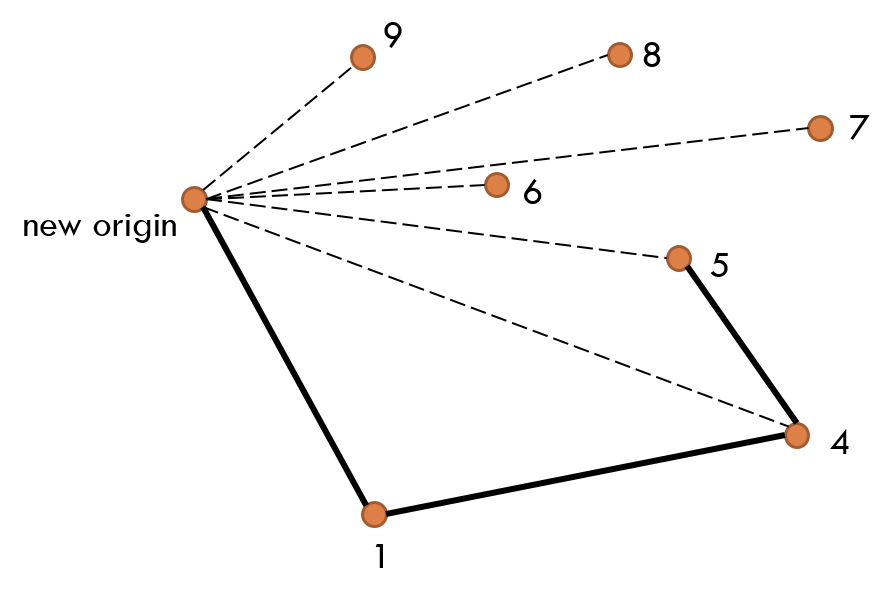
\includegraphics[height=0.5\textheight]{figures/graham7}
\end{center}
\end{frame}

\begin{frame}{Example}
Continue adding points...
\begin{center}
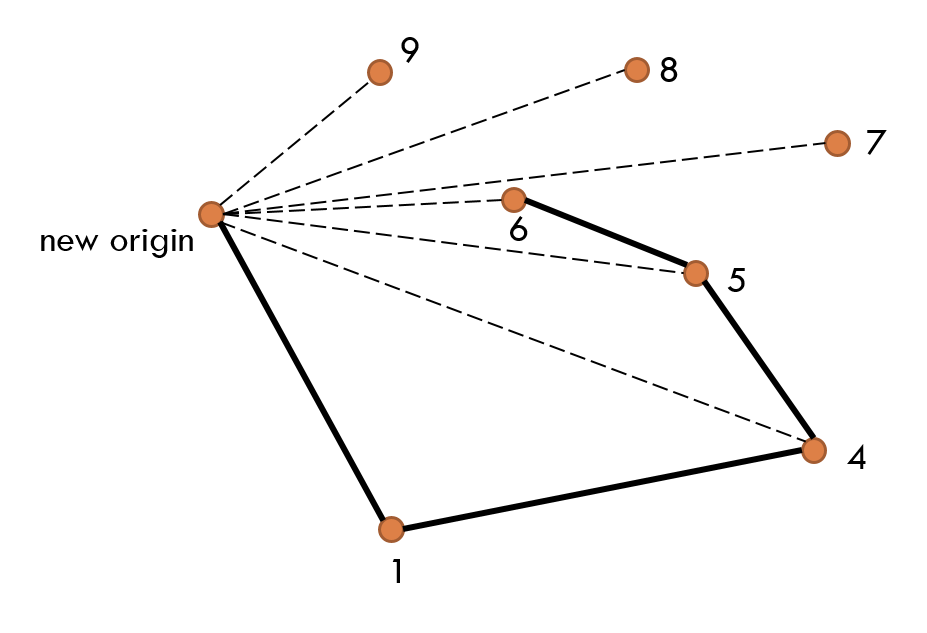
\includegraphics[height=0.5\textheight]{figures/graham8}
\end{center}
\end{frame}

\begin{frame}{Example}
Bad corner!
\begin{center}
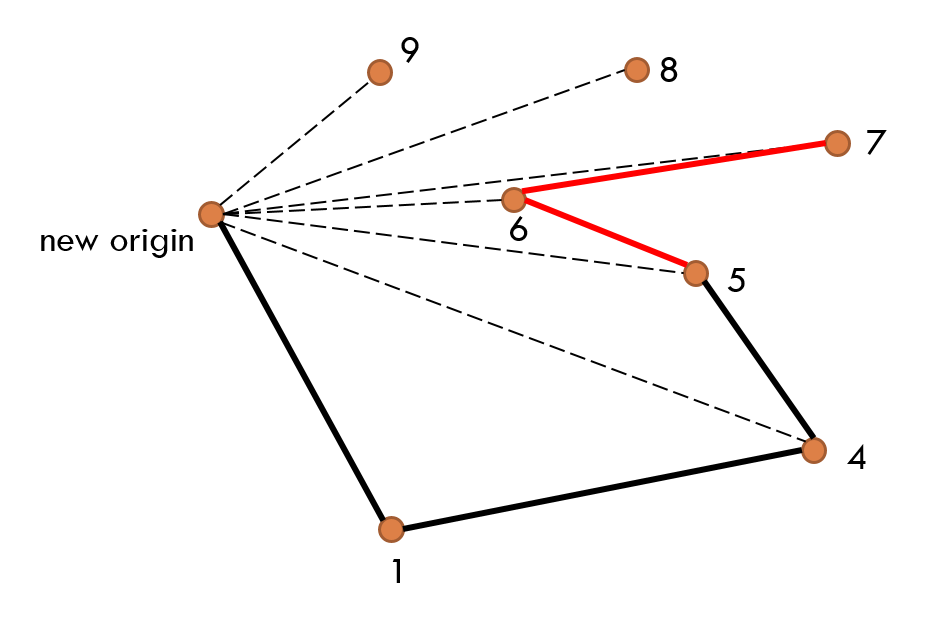
\includegraphics[height=0.5\textheight]{figures/graham9}
\end{center}
\end{frame}

\begin{frame}{Example}
Bad corner again!
\begin{center}
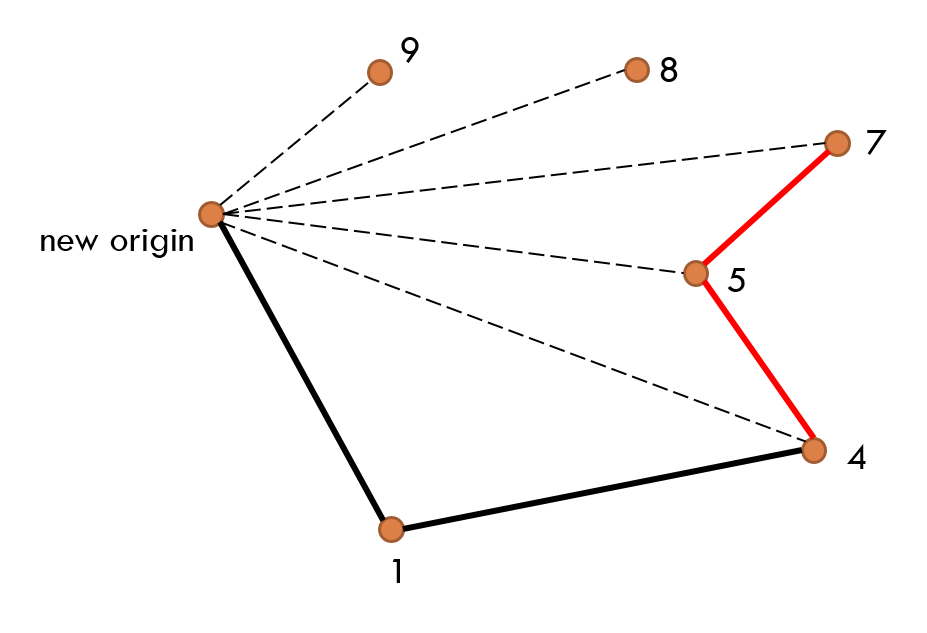
\includegraphics[height=0.5\textheight]{figures/graham10}
\end{center}
\end{frame}

\begin{frame}{Example}
Continue adding points...
\begin{center}
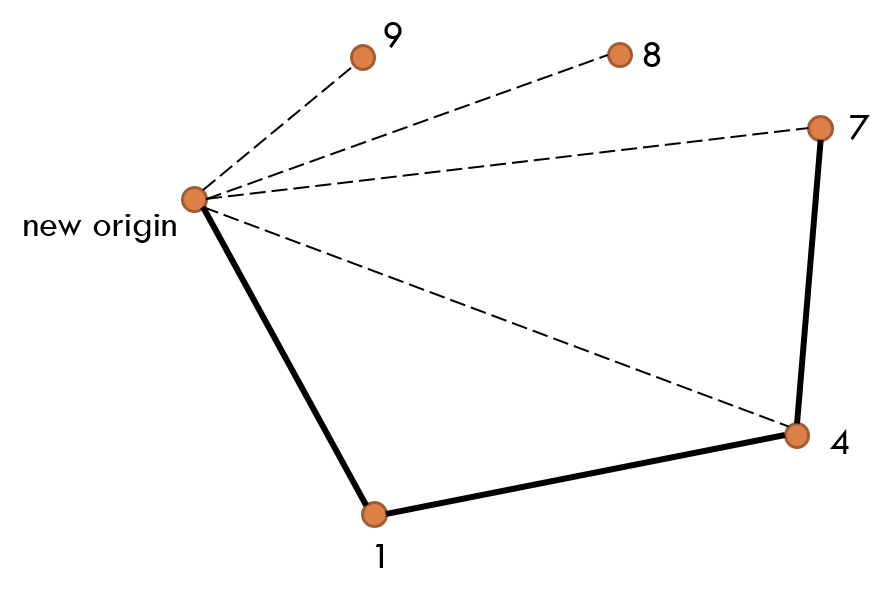
\includegraphics[height=0.5\textheight]{figures/graham11}
\end{center}
\end{frame}

\begin{frame}{Example}
Continue adding points...
\begin{center}
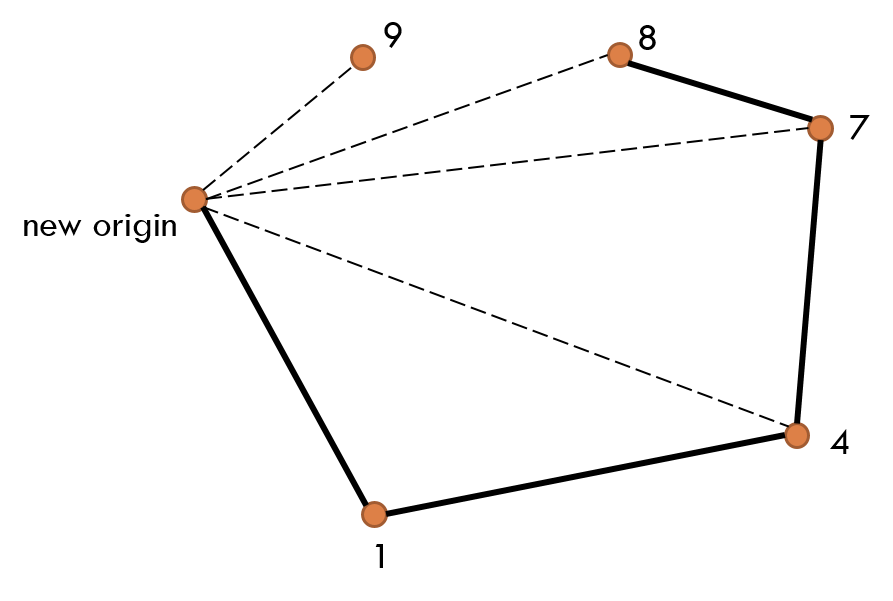
\includegraphics[height=0.5\textheight]{figures/graham12}
\end{center}
\end{frame}

\begin{frame}{Example}
Continue adding points...
\begin{center}
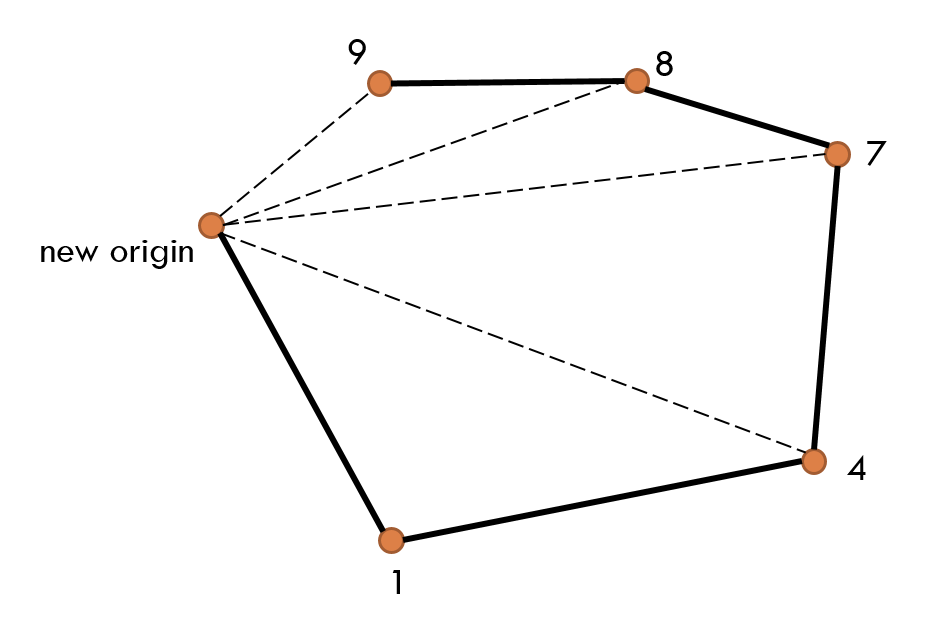
\includegraphics[height=0.5\textheight]{figures/graham13}
\end{center}
\end{frame}

\begin{frame}{Example}
Done!
\begin{center}
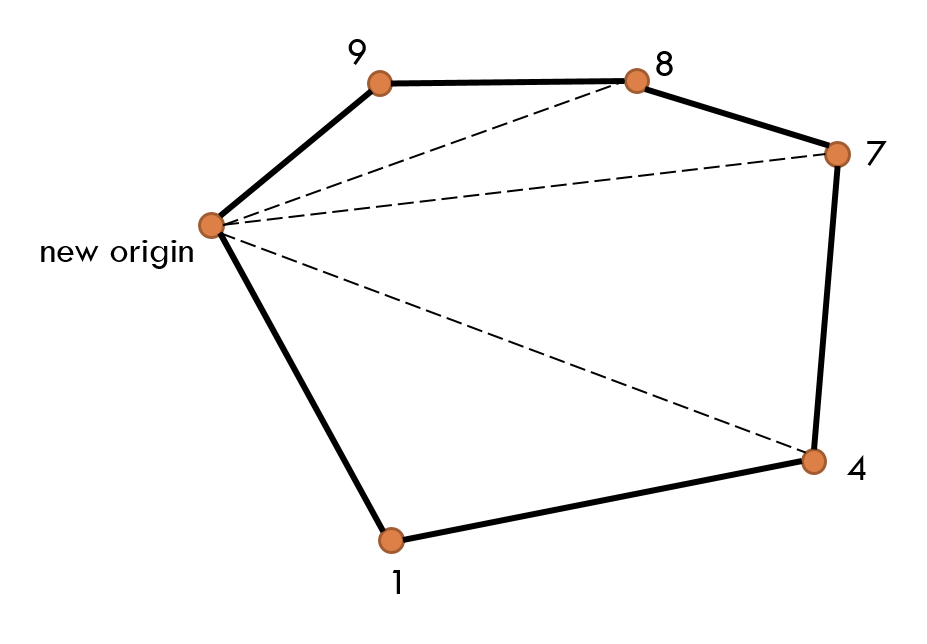
\includegraphics[height=0.5\textheight]{figures/graham14}
\end{center}
\end{frame}

\begin{frame}{Pseudocode}
\BIT
\item Set the leftmost point as $(0, 0)$, and sort the rest of the points in increasing order of $y/x$
\item Initialize stack $S$
\item For $i=1, \ldots, n$:
\BIT
\item Let $A$ be the second topmost element of $S$, $B$ be the topmost element of $S$, and $C$ be the $i$th point
\item If $\mathrm{ccw}(A, B, C) < 0$, pop $S$ and go back
\item Push $C$ to $S$
\EIT
\item Points in $S$ form the convex hull
\EIT
\end{frame}

\section{Sweep Line Algorithm}

\begin{frame}{Sweep Line Algorithm}
\BIT
\item A problem solving strategy for geometry problems
\item The main idea is to maintain a line (with some auxiliary data structure) that sweeps through the entire plane and solve the problem locally
\item We can't simulate a continuous process, (e.g. sweeping a line) so we define events that causes certain changes in our data structure
\BIT
\item And process the events in the order of occurrence
\EIT
\item We'll cover one sweep line algorithm
\EIT
\end{frame}

\begin{frame}{Sweep Line Algorithm}
\BIT
\item Problem: Given $n$ axis-aligned rectangles, find the area of the union of them
\item We will sweep the plane from left to right
\item Events: left and right edges of the rectangles
\item The main idea is to maintain the set of ``active'' rectangles in order
\BIT
\item It suffices to store the $y$-coordinates of the rectangles
\EIT \EIT
\end{frame}

\begin{frame}{Example}
\begin{center}
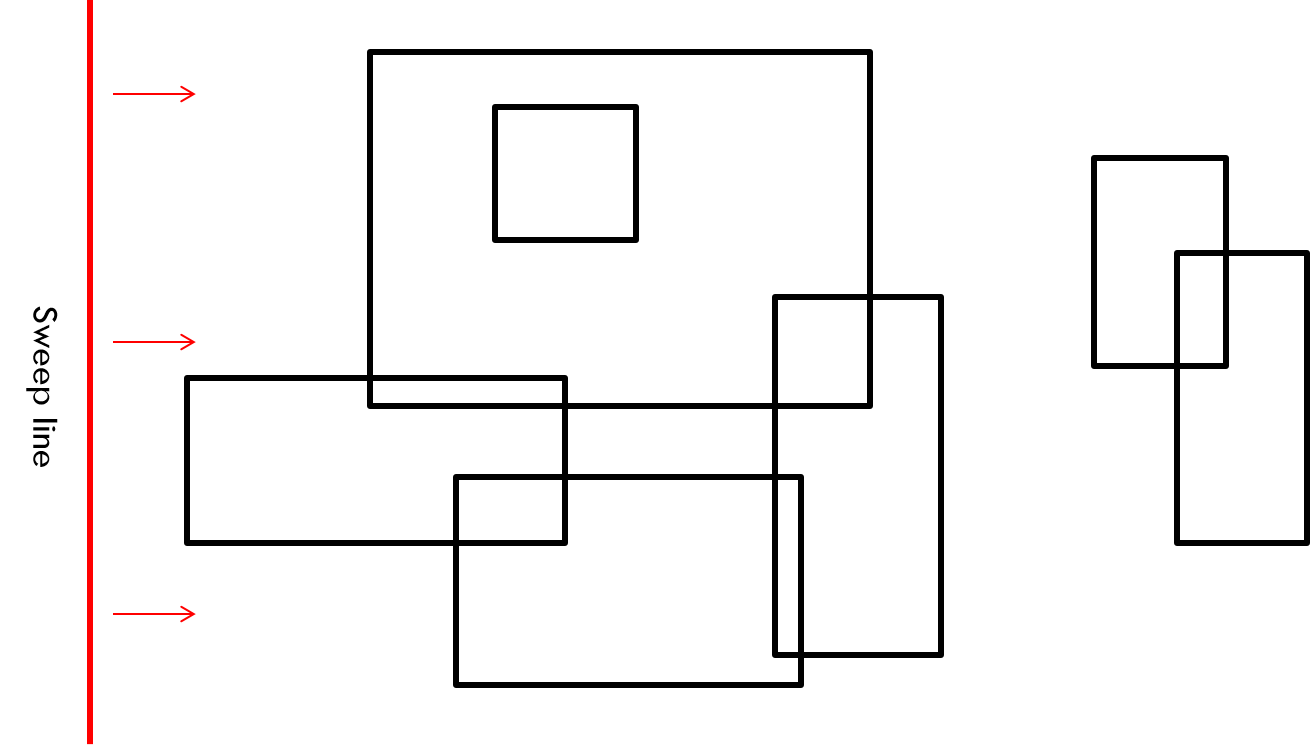
\includegraphics[height=0.6\textheight]{figures/sweep1}
\end{center}
\end{frame}

\begin{frame}{Example}
\begin{center}
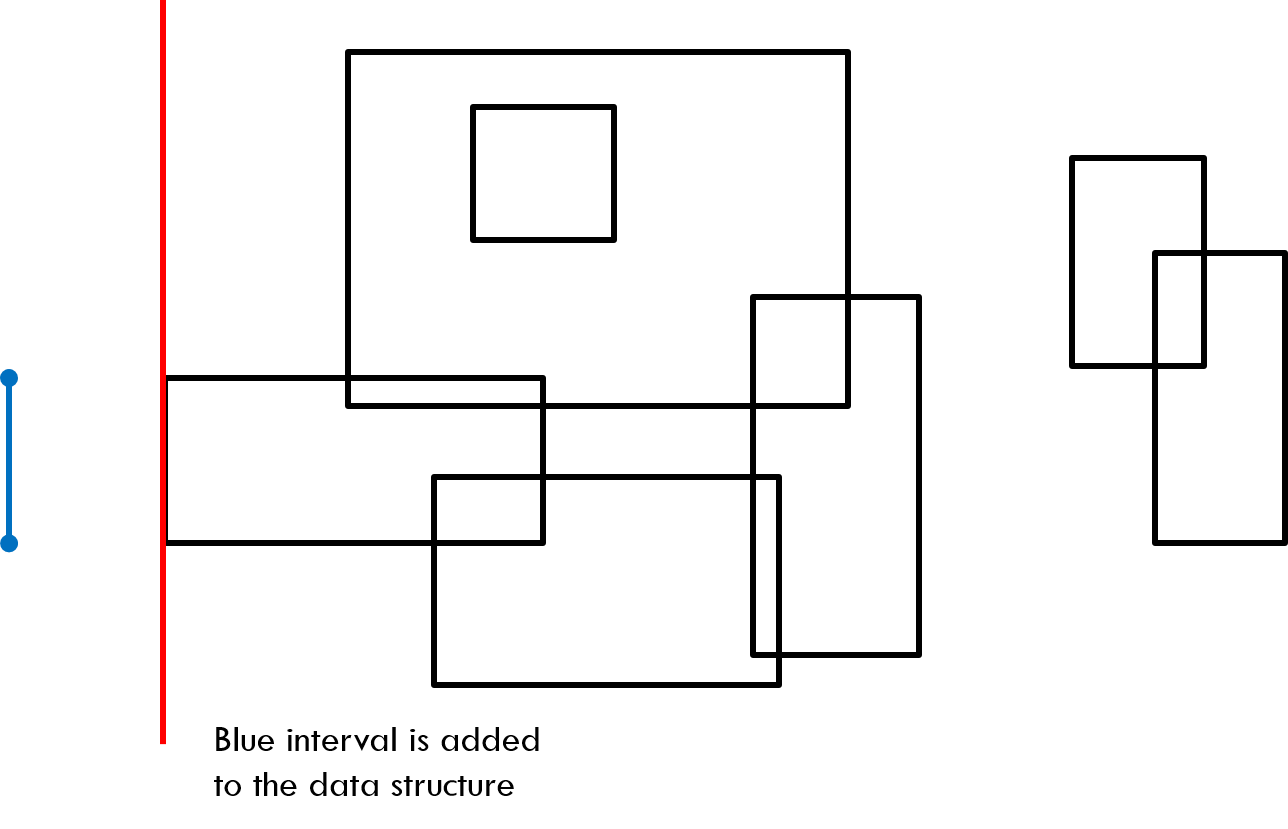
\includegraphics[height=0.6\textheight]{figures/sweep2}
\end{center}
\end{frame}

\begin{frame}{Example}
\begin{center}
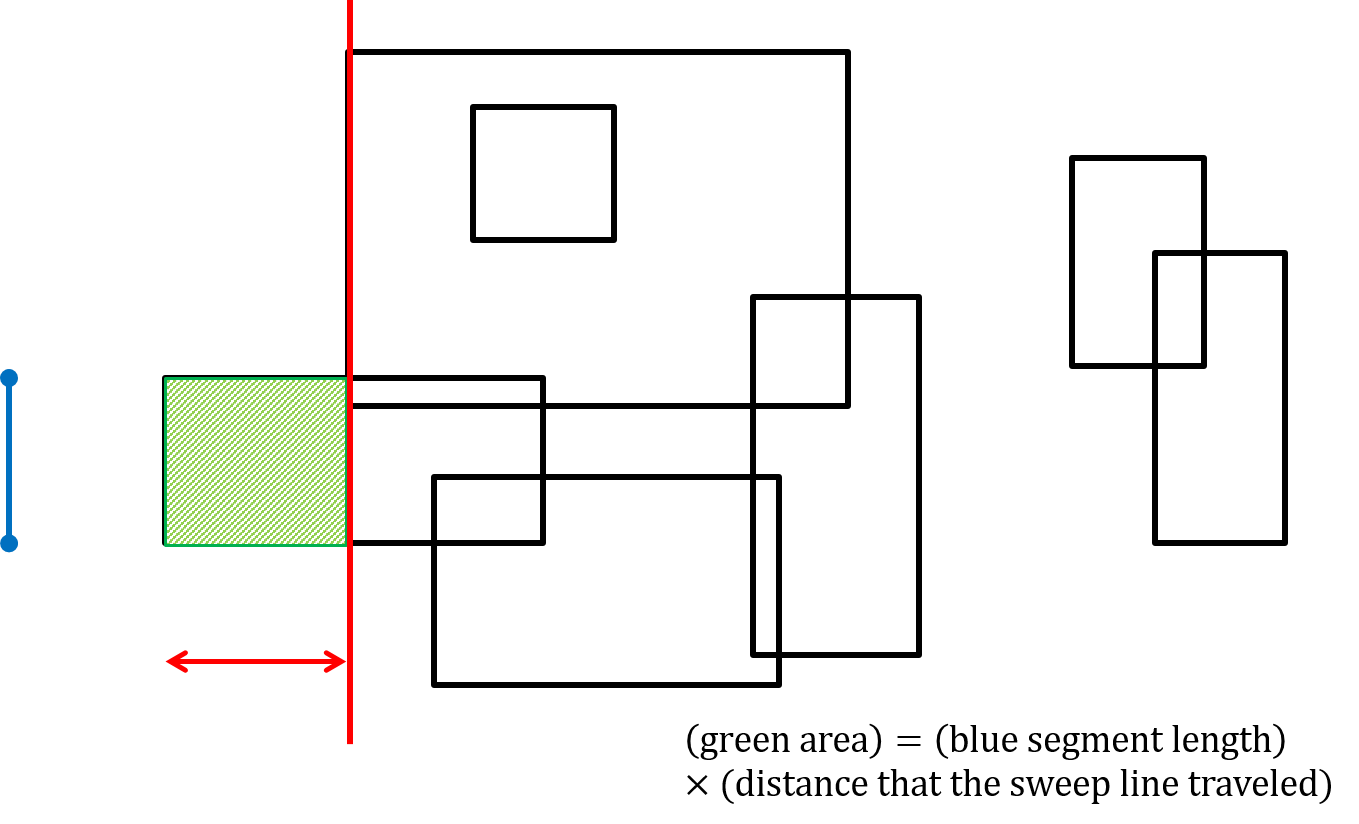
\includegraphics[height=0.6\textheight]{figures/sweep3}
\end{center}
\end{frame}

\begin{frame}{Example}
\begin{center}
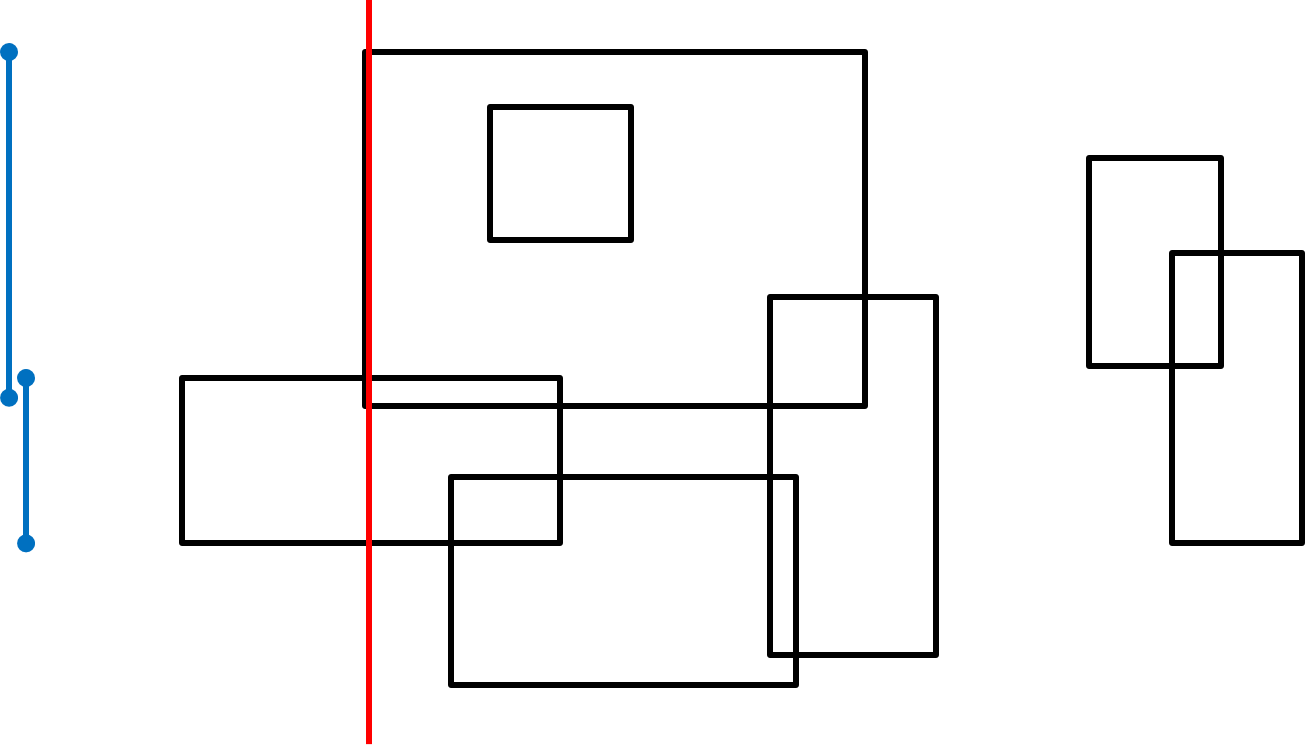
\includegraphics[height=0.6\textheight]{figures/sweep4}
\end{center}
\end{frame}

\begin{frame}{Example}
\begin{center}
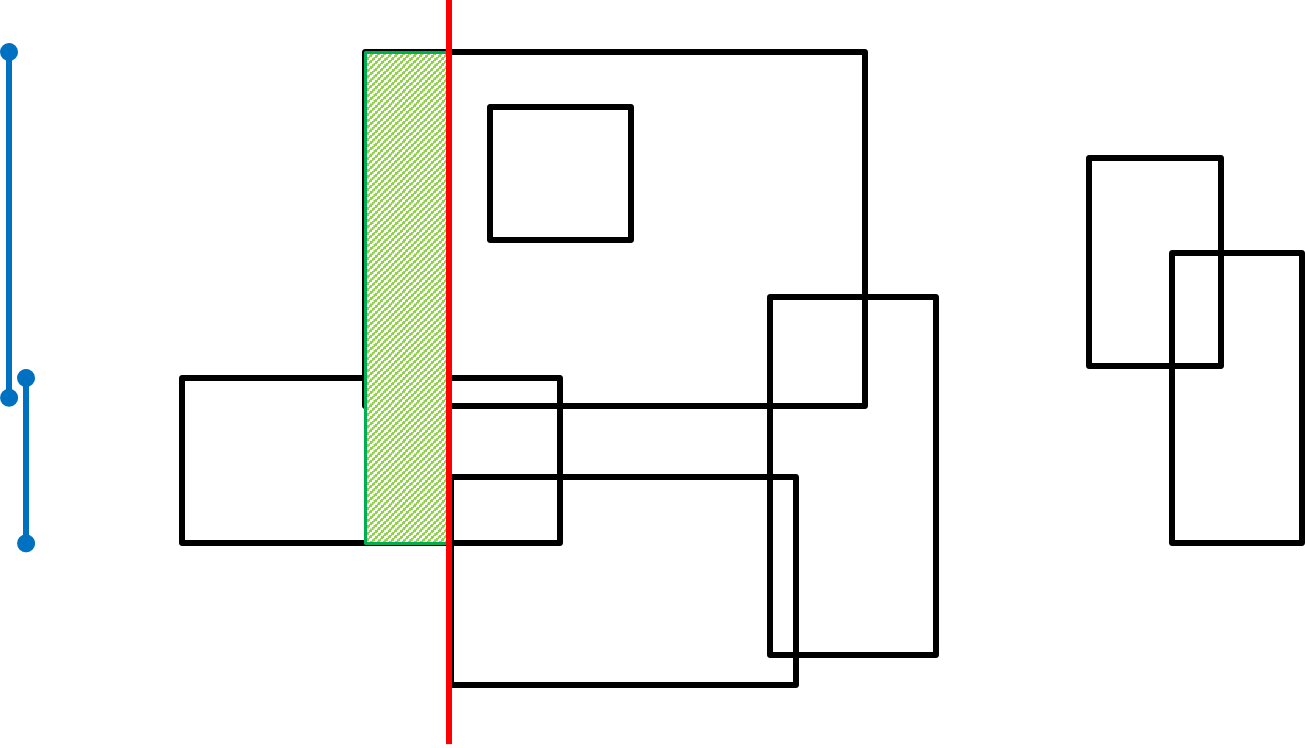
\includegraphics[height=0.6\textheight]{figures/sweep5}
\end{center}
\end{frame}

\begin{frame}{Example}
\begin{center}
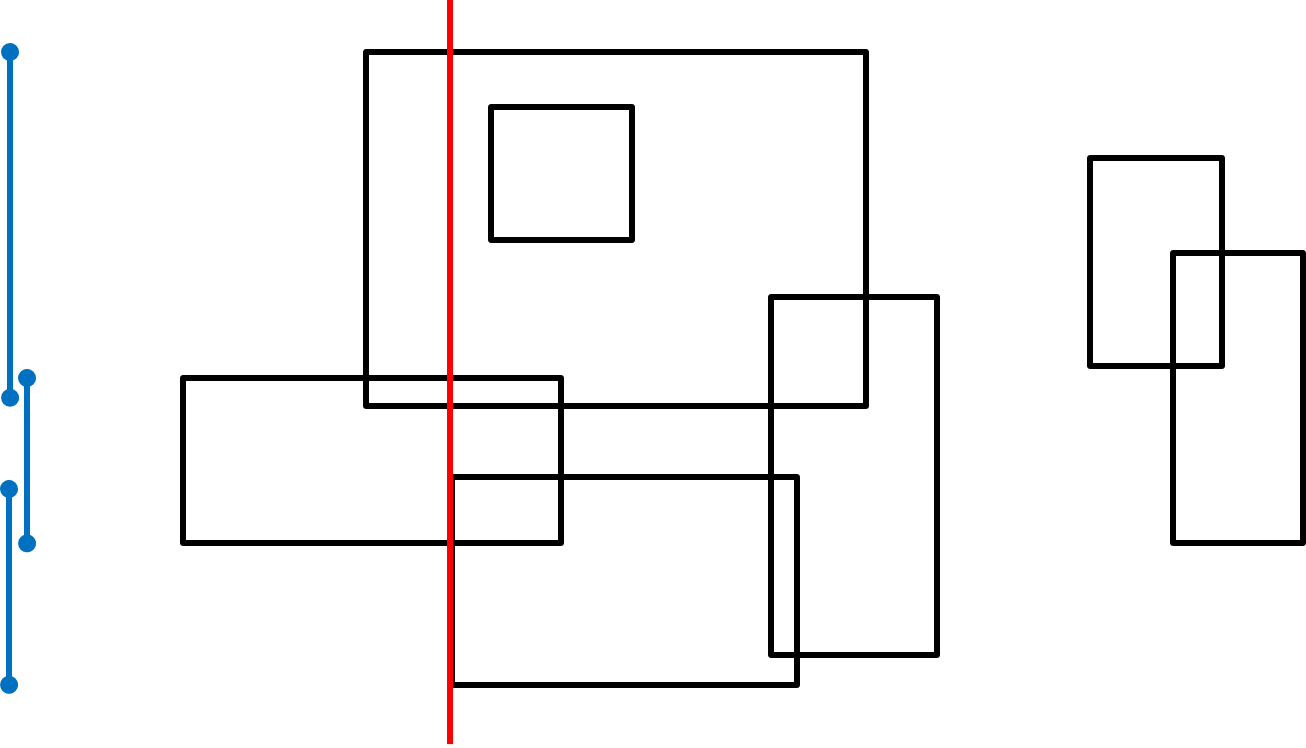
\includegraphics[height=0.6\textheight]{figures/sweep6}
\end{center}
\end{frame}

\begin{frame}{Example}
\begin{center}
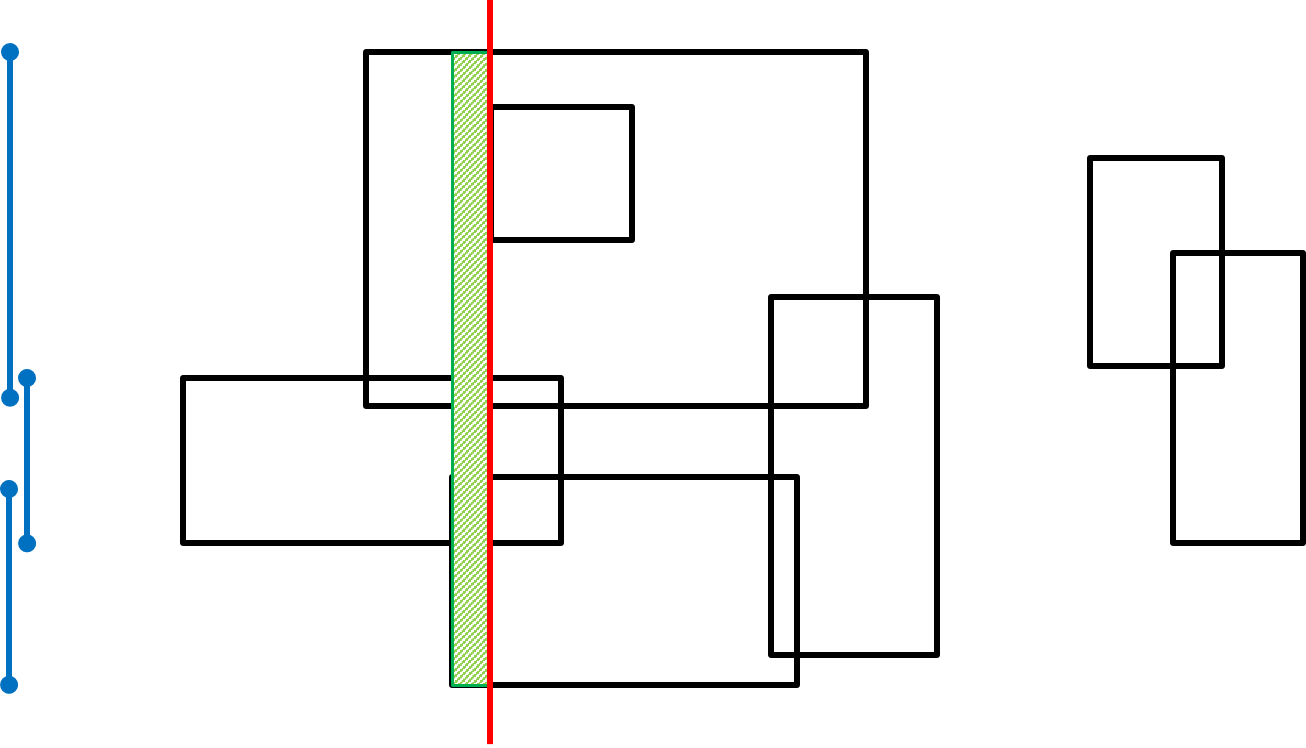
\includegraphics[height=0.6\textheight]{figures/sweep7}
\end{center}
\end{frame}

\begin{frame}{Example}
\begin{center}
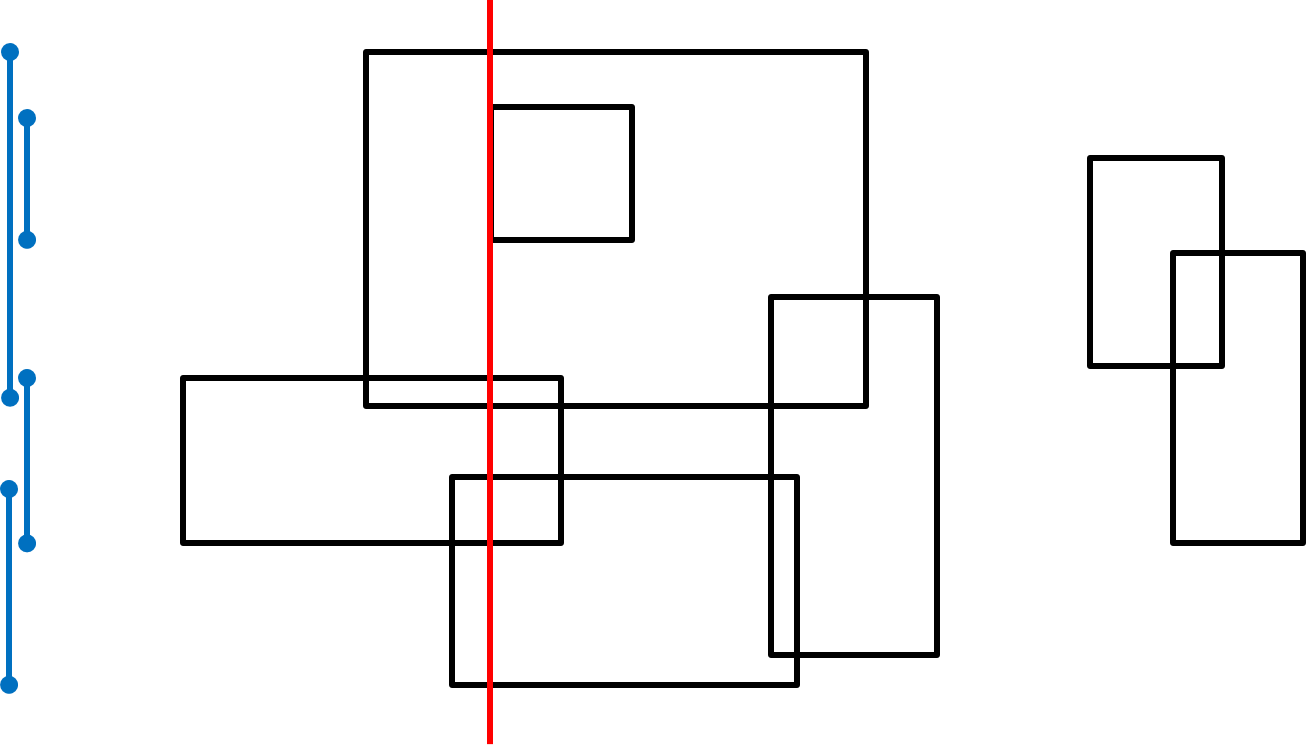
\includegraphics[height=0.6\textheight]{figures/sweep8}
\end{center}
\end{frame}

\begin{frame}{Example}
\begin{center}
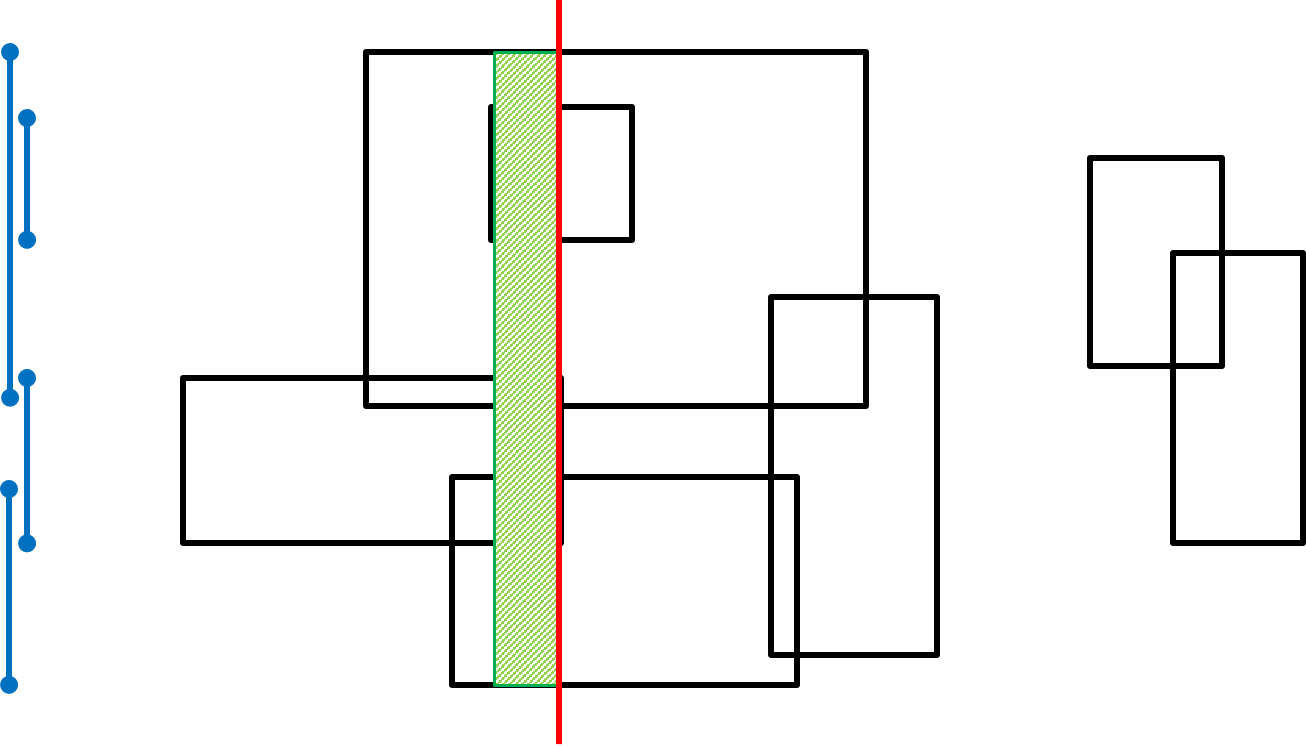
\includegraphics[height=0.6\textheight]{figures/sweep9}
\end{center}
\end{frame}

\begin{frame}{Example}
\begin{center}
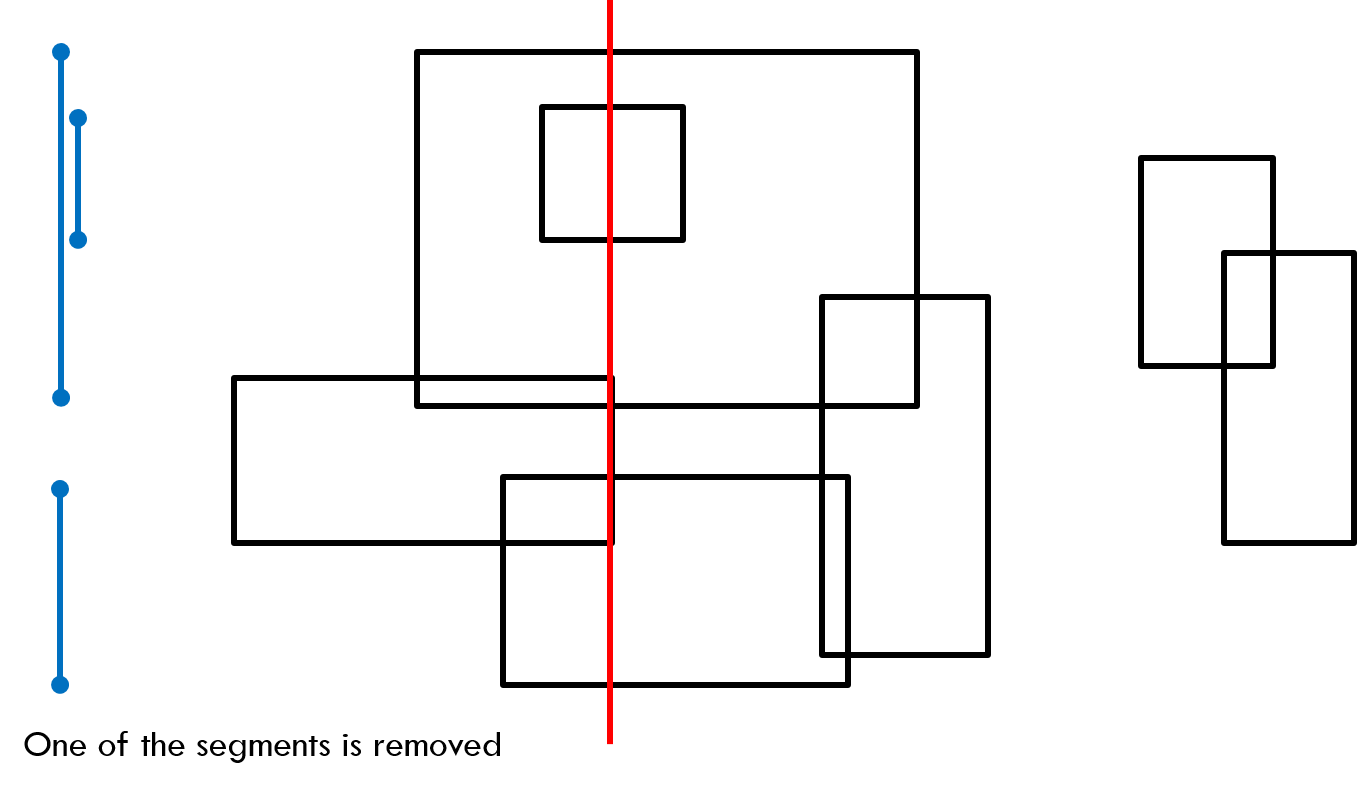
\includegraphics[height=0.6\textheight]{figures/sweep10}
\end{center}
\end{frame}

\begin{frame}{Example}
\begin{center}
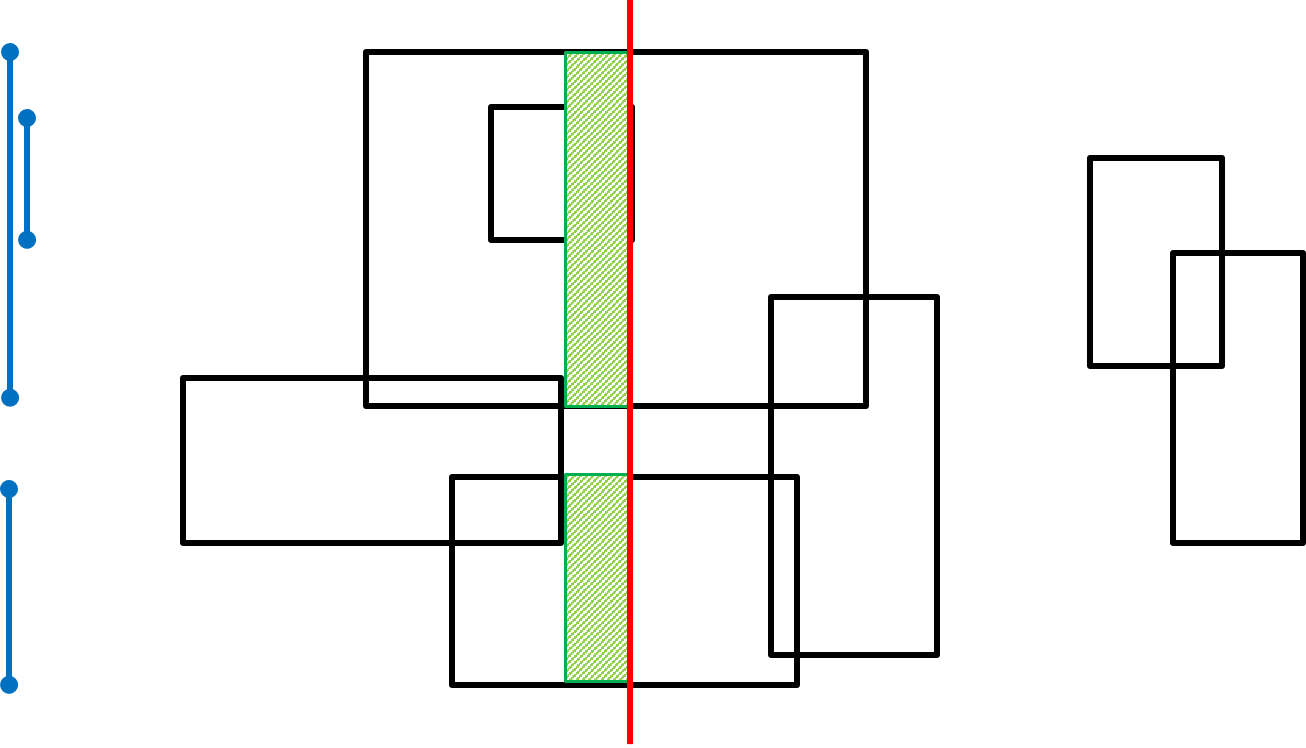
\includegraphics[height=0.6\textheight]{figures/sweep11}
\end{center}
\end{frame}

\begin{frame}{Pseudo-pseudocode}
\BIT
\item If the sweep line hits the left edge of a rectangle
\BIT
\item Insert it to the data structure
\EIT
\item Right edge?
\BIT
\item Remove it
\EIT
\item Move to the next event, and add the area(s) of the green rectangle(s)
\BIT
\item Finding the length of the union of the blue segments is the hardest step
\item There is an easy $O(n)$ method for this step
\EIT
\EIT
\end{frame}

\begin{frame}{Notes on Sweep Line Algorithms}
\BIT
\item Sweep line algorithm is a generic concept
\BIT
\item Come up with the right set of events and data structures for each problem
\EIT
\item Exercise problems
\BIT
\item Finding the perimeter of the union of rectangles
\item Finding all $k$ intersections of $n$ line segments in $O((n+k) \log n)$ time
\EIT\EIT
\end{frame}

\section{Intersecting Half-planes}

\begin{frame}{Intersecting Half-planes}
\BIT
\item Representing a half-plane: $ax+by+c \le 0$
\item The intersection of half-planes is a convex area
\BIT
\item If the intersection is bounded, it gives a convex polygon
\EIT
\item Given $n$ half-planes, how do we compute the intersection of them?
\BIT
\item \ie, Find vertices of the convex area
\EIT
\item There is an easy $O(n^3)$ algorithm and a hard $O(n \log n)$ one
\BIT
\item We will cover the easy one
\EIT\EIT
\end{frame}

\begin{frame}{Intersecting Half-planes}
\BIT
\item For each half-plane $a_ix + b_iy + c_i \le 0$, define a straight line $e_i: a_ix + b_iy + c_i = 0$
\item For each pair of $e_i$ and $e_j$:
\BIT
\item Compute their intersection $p=(p_x, p_y)$
\item Check if $a_k p_x + b_k p_y + c_k \le 0$ for all half-planes
\BIT
\item If so, store $p$ in some array $P$
\item Otherwise, discard $p$
\EIT\EIT
\item Find the convex hull of the points in $P$
\EIT
\end{frame}

\begin{frame}{Intersecting Half-planes}
\BIT
\item The intersection of half-planes can be unbounded
\BIT
\item But usually, we are given limits on the min/max values of the coordinates
\item Add four half-planes $x \ge -M$, $x \le M$, $y \ge -M$, $y \le M$ (for large $M$) to ensure that the intersection is bounded
\EIT
\item Time complexity: $O(n^3)$
\BIT
\item Pretty slow, but easy to code
\EIT\EIT
\end{frame}

\section{Notes on Binary/Ternary Search}

\begin{frame}{Notes on Binary Search}
\BIT
\item Usually, binary search is used to find an item ofi rulnterest in a sorted array
\vfill
\item There is a nice application of binary search, often used in geometry problems
\BIT
\item Example: finding the largest circle that fits into a given polygon
\BIT
\item Don't try to find a closed form solution or anything like that!
\item Instead, binary search on the answer
\EIT\EIT
\EIT
\end{frame}

\begin{frame}{Ternary Search}
\BIT
\item Another useful method in many geometry problems
\item Finds the minimum point of a ``convex'' function $f$
\BIT
\item Not exactly convex, but let's use this word anyway
\EIT
\item Initialize the search interval $[s, e]$
\item Until $e-s$ becomes ``small enough'':
\BIT
\item $m_1 := s+(e-s)/3$, $m_2 := e - (e-s)/3$
\item If $f(m_1) \le f(m_2)$, set $e := m_2$
\item Otherwise, set $s := m_1$
\EIT\EIT
\end{frame}

\end{document}
